\subsection {Ripple Counters}

Tipicamente, esses contadores são implementados com flip-flops JK ou D conectados em cascata, conforme ilustrado a seguir:

\begin{figure}[H]
   	\centering
   	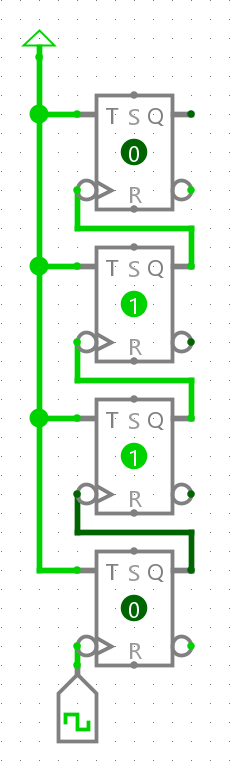
\includegraphics[width=0.14\linewidth]{images/assincrono-circuit.png}
  	 \caption{Circuito de um contador assíncrono}
   	\label{fig:assincrono-circuit}
\end{figure}


\textbf{increase/decrease} e borda do clock